\chapter{Implementation Detail}
\label{app:impl}

This appendix holds the implementation detail of the design summarised in Chapter~\ref{chap:design}: pin and bus assignments, task and queue structure, line and record formats, parameters, thresholds and the history of each part across firmware versions. The sections follow the order of that chapter. The firmware configuration is in Table~\ref{tab:config} (Appendix~\ref{app:devrecord}) and every connection in Appendix~\ref{app:wiring}.

\section{Hardware}
\label{sec:impl-hardware}

In the first bench versions the Raspberry Pi~4 faced forward and the dashboard read it over Wi-Fi; the first camera went on the Raspberry Pi~4 rather than the Raspberry Pi~5 because the Pi~5 ran the inherited dashboard, and developing on it would have put a working deployment at risk. The two-sided layout of Section~\ref{sec:two-sided} replaced this on 15 October, and until 21 October the rear unit's link to the Raspberry Pi~4 was USB (Section~\ref{sec:impl-comms}).

The telemetry unit is a Makerfabs ESP32-S3 4G LTE CAT1 A7670X board: an ESP32-S3-WROOM-1-N16R8 module (16\,MB flash, 8\,MB PSRAM) with an A7670X LTE Cat-1 modem that also contains the GNSS receiver \cite{makerfabsa7670x} (Figure~\ref{fig:makerfabs-pinout}, Appendix~\ref{app:figures}). The integrated board lets processor, modem and GNSS be tested without a separate modem circuit. Up to 22 October two MPU6050 IMUs were on separate I\textsuperscript{2}C buses at 400\,kHz (GPIO8/9 and GPIO17/18), which avoids their shared address and bus contention; since then the board carries IMU1 only, on GPIO8/9, and the second sensor is on the front node. The modem is on a hardware UART at 115200\,bit/s, with its power key and reset on GPIO~4 and~5. The unit's lines go to the Raspberry Pi~4 on the spare pins IO41 and IO42 (Section~\ref{sec:pi-link}). The board's microSD slot was not used: its chip-select line passes through a resistor (R23) that the schematic marks as not fitted, so local logging uses the internal flash (Section~\ref{sec:local-logging}).

Each camera unit carries an OV5647 camera module without an infrared-cut filter and three VL53L0X time-of-flight sensors on its I\textsuperscript{2}C bus: the Raspberry Pi~5 beside the display faces forward, and the Raspberry Pi~4 beside the battery faces backward and also takes the sync-pulse input on GPIO17 (Section~\ref{sec:two-sided}). The Raspberry Pi~4's camera is on a 15\,cm ribbon. Each camera is housed in a three-part casing designed and 3D printed in this project (Figure~\ref{fig:camera-casing}, Appendix~\ref{app:figures}), not yet fixed to the vehicle. The enclosures and mounts designed to put the system on the vehicle (the dashboard display mount, the two sensor pods and the IMU pods), the choices behind them and the checks on their geometry are in Appendix~\ref{app:mechanical}; none had been printed by 12 October. Every connection is listed in Appendix~\ref{app:wiring}, and Figure~\ref{fig:bench-setup} shows the bench setup.

\begin{figure}[htbp]
\centering
\begin{tikzpicture}[
  lbl/.style={font=\footnotesize, text width=3.5cm, inner sep=1pt},
  pin/.style={draw=black, fill=white, circle, inner sep=0pt, minimum size=4.5pt},
  lead/.style={line width=0.6pt, draw=black, preaction={draw=white, line width=2.2pt}}]
\node[anchor=south west, inner sep=0] (img) at (0,0) {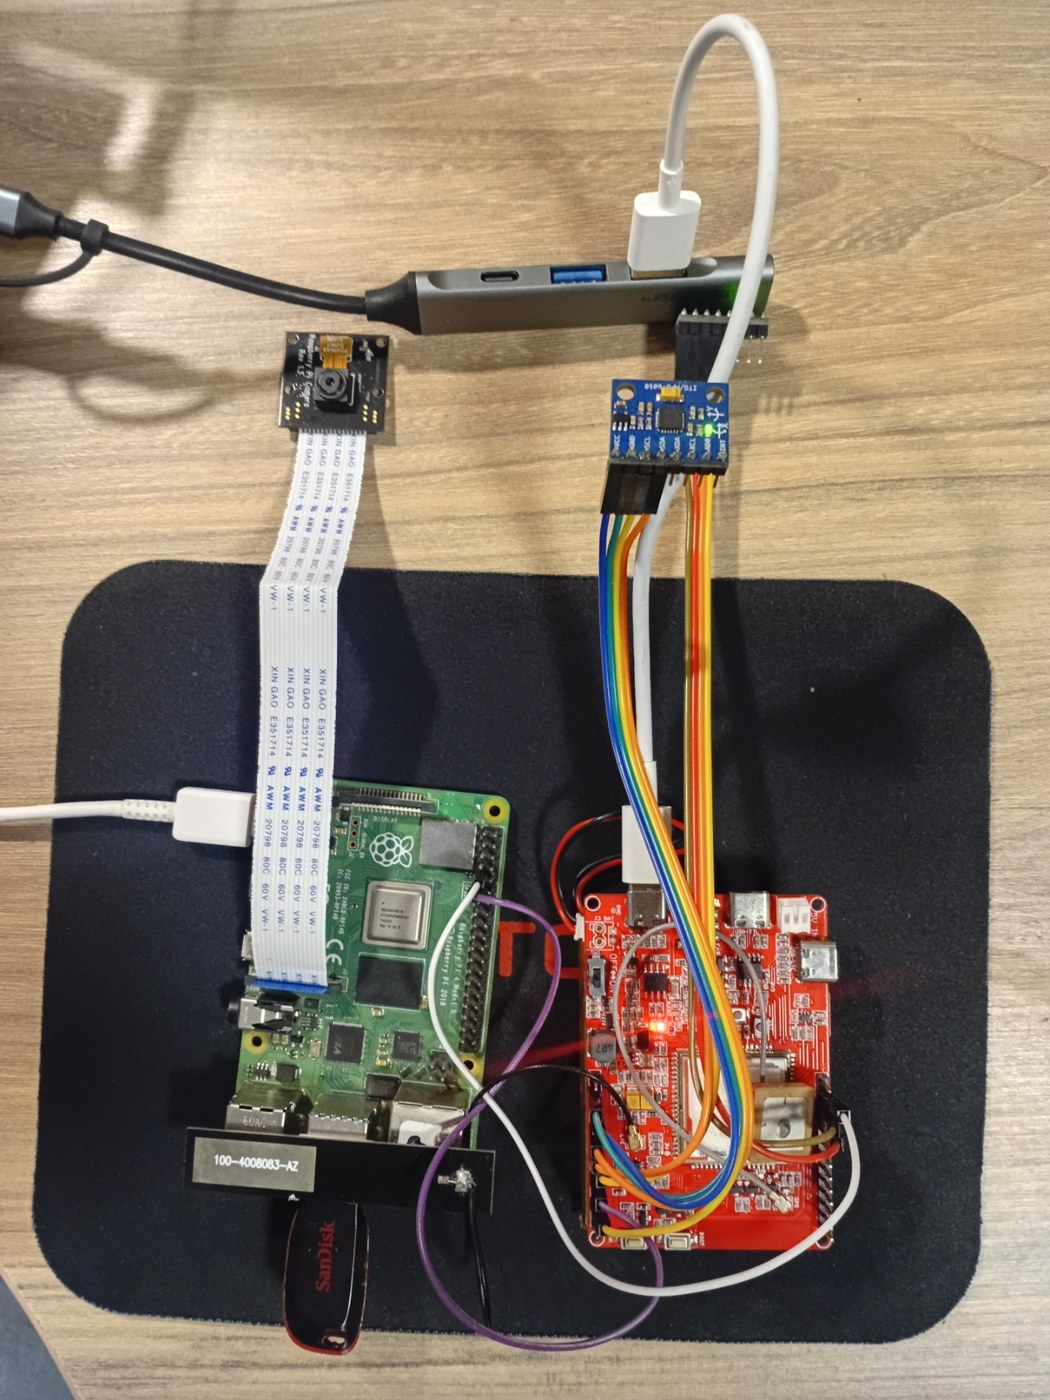
\includegraphics[width=0.45\textwidth]{figures/bench_setup.jpg}};
\begin{scope}[x={(img.south east)}, y={(img.north west)}]
  \node[lbl, anchor=east, align=right] (cam) at (-0.04,0.73) {OV5647 camera};
  \node[lbl, anchor=east, align=right] (syn) at (-0.04,0.53) {Sync-pulse wire, ESP32 GPIO15 to Pi GPIO17};
  \node[lbl, anchor=east, align=right] (pi)  at (-0.04,0.35) {Raspberry Pi 4: camera, sync logging, detection};
  \node[lbl, anchor=east, align=right] (lte) at (-0.04,0.18) {LTE antenna};
  \node[lbl, anchor=east, align=right] (usb) at (-0.04,0.02) {USB boot drive for the Pi};
  \node[lbl, anchor=west, align=left] (hub) at (1.04,0.82) {USB hub};
  \node[lbl, anchor=west, align=left] (imu) at (1.04,0.64) {MPU6050 IMU, 200\,Hz};
  \node[lbl, anchor=west, align=left] (esp) at (1.04,0.40) {ESP32-S3 and A7670X board: acquisition, features, BMS, GNSS, logging, LTE};
  \node[lbl, anchor=west, align=left] (gps) at (1.04,0.15) {GNSS patch antenna};
  \draw[lead] (cam.east) -- (0.32,0.73); \node[pin] at (0.32,0.73) {};
  \draw[lead] (syn.east) -- (0.45,0.37); \node[pin] at (0.45,0.37) {};
  \draw[lead] (pi.east)  -- (0.38,0.28); \node[pin] at (0.38,0.28) {};
  \draw[lead] (lte.east) -- (0.24,0.17); \node[pin] at (0.24,0.17) {};
  \draw[lead] (usb.east) -- (0.31,0.09); \node[pin] at (0.31,0.09) {};
  \draw[lead] (hub.west) -- (0.55,0.79); \node[pin] at (0.55,0.79) {};
  \draw[lead] (imu.west) -- (0.63,0.70); \node[pin] at (0.63,0.70) {};
  \draw[lead] (esp.west) -- (0.66,0.28); \node[pin] at (0.66,0.28) {};
  \draw[lead] (gps.west) -- (0.745,0.20); \node[pin] at (0.745,0.20) {};
\end{scope}
\end{tikzpicture}
\caption{Bench setup of the telemetry system before the two-sided layout, each component labelled by its role. At this stage the Raspberry Pi~4 carried the only camera; in the final layout it is the rear unit and the Raspberry Pi~5 carries the front camera (Figure~\ref{fig:two-sided}).}
\label{fig:bench-setup}
\end{figure}

\section{Firmware tasks and acquisition}
\label{sec:impl-fw}

The firmware is written with PlatformIO and the Arduino framework on FreeRTOS (Table~\ref{tab:config}); one source builds both nodes. Figure~\ref{fig:task-architecture} shows its tasks and queues. Each IMU task runs at the highest priority on core~1 and holds a 5\,ms period with \texttt{vTaskDelayUntil}, which schedules each wake-up from the previous target time so that variable execution time does not accumulate into drift. After a stall it returns at once for each missed period, so the missed samples are read in a burst about 1\,ms apart: none is lost, but they are unevenly spaced. Since v0.7.6 a task more than 20 periods (100\,ms) behind gives up the missed slots and counts them as late, so a slow bus cannot hold the core; the 33 to 44\,ms flash-write pause is still caught up as before (Section~\ref{sec:buffering}). The modem, BMS and dashboard-line tasks run on core~0. Up to v0.7.5 the statistics and ride-feature tasks ran on core~1 below the IMU tasks; v0.7.6 moved them to core~0 at priority~2, above every other task there, after the consumer-stall fault (Section~\ref{sec:inv-stall}), so core~1 now holds only the IMU tasks and the sync task.

\begin{figure}[htbp]
\centering
% FreeRTOS tasks and queues, firmware v0.7.1. Source: TelemetryUnit/src/main.cpp, setup() (queues
% lines 2376 to 2381, tasks lines 2391 to 2411); StatsTask reports every 2 s, SyncTask toggles every
% 500 ms, the ride windows are 1 s (RIDE_WINDOW_SAMPLES = 200), ModemTask polls GNSS every 3 s and
% builds, logs and publishes the telemetry record every 10 s.
\begin{tikzpicture}[x=1cm, y=1cm]
  \def\tw{4.0cm}
  \def\tn{2.6cm}
  % ---- core 0 ----
  \node[swbox, text width=\tw] (modem) at (2.4,-1.1) {\textbf{ModemTask}, priority 1\\ AT commands; GNSS every 3\,s;\\ every 10\,s: flash log and MQTT};
  \node[swbox, text width=\tw] (bms) at (2.4,-3.0) {\textbf{BmsTask}, priority 1\\ battery frames over BLE};
  \node[swbox, text width=\tw] (hall) at (2.4,-4.6) {\textbf{HallTask}, priority 1\\ pulse counter, read every 1\,s};
  \node[swbox, text width=\tw] (dash) at (2.4,-6.2) {\textbf{DashTask}, priority 1\\ \texttt{DASH} line on USB, every 1\,s};
  % ---- core 1 ----
  \node[swbox, text width=3.6cm] (stats) at (10.6,-1.1) {\textbf{StatsTask}, priority 2\\ rates, jitter, drops every 2\,s};
  \node[swbox, text width=\tn] (imu1) at (7.6,-3.0) {\textbf{Imu1Task}\\ priority 3, 200\,Hz};
  \node[swbox, text width=\tn] (imu2) at (13.6,-3.0) {\textbf{Imu2Task}\\ priority 3, 200\,Hz};
  \node[swbox, text width=\tn] (ride1) at (7.6,-4.9) {\textbf{RideChar1Task}\\ priority 1, 1\,s windows};
  \node[swbox, text width=\tn] (ride2) at (13.6,-4.9) {\textbf{RideChar2Task}\\ priority 1, 1\,s windows};
  \node[swbox, fill=white, text width=3.6cm] (fuse) at (10.6,-6.4) {Dual-IMU fusion: pairs the two windows};
  \node[swbox, text width=3.6cm] (sync) at (10.6,-7.8) {\textbf{SyncTask}, priority 2\\ toggles GPIO15 every 500\,ms};
  % ---- lanes ----
  \begin{scope}[on background layer]
    \coordinate (t0) at (0.3,-0.25); \coordinate (b0) at (0.3,-8.45);
    \coordinate (t1) at (6.2,-0.25); \coordinate (b1) at (6.2,-8.45);
    \node[swlane, fit=(modem)(bms)(hall)(dash)(t0)(b0)] (c0) {};
    \node[swlane, fit=(stats)(imu1)(imu2)(ride1)(ride2)(fuse)(sync)(t1)(b1)] (c1) {};
  \end{scope}
  \node[swlanetitle] at (c0.north west) {Core 0: communication};
  \node[swlanetitle] at (c1.north west) {Core 1: acquisition and processing};
  % ---- queues (labels give name and capacity) ----
  \draw[swflow] (imu1.north) -- node[swlabel, pos=0.45, left=2pt] {\texttt{imu1Queue}, 100} (stats.south west);
  \draw[swflow] (imu2.north) -- node[swlabel, pos=0.45, right=2pt] {\texttt{imu2Queue}, 100} (stats.south east);
  \draw[swflow] (imu1) -- node[swlabel, right=2pt] {\texttt{imu1CharQueue}, 400} (ride1);
  \draw[swflow] (imu2) -- node[swlabel, left=2pt] {\texttt{imu2CharQueue}, 400} (ride2);
  \draw[swflow] (ride1.south) |- (fuse.west);
  \draw[swflow] (ride2.south) |- (fuse.east);
  \draw[swlink] ($(modem.east)+(0,0.25)$) -- node[swlabel, above=1pt] {\texttt{gnssQueue}, 20} ($(stats.west)+(0,0.25)$);
  \draw[swlink] (bms.east) -- (5.45,-3.0) |- node[swlabel, pos=0.75, below=1pt] {\texttt{bmsQueue}, 20} ($(stats.west)+(0,-0.25)$);
\end{tikzpicture}

\caption{FreeRTOS tasks and queues as drawn for firmware v0.7.1 and unchanged to v0.7.4.1. Priorities as set in the firmware (higher runs first); each queue is labelled with its name and capacity in items. Queues between the two cores are drawn in blue. Later changes, not drawn: the raw-stream sender (v0.7.5), the statistics and ride tasks moved to core~0 at priority~2 (v0.7.6), the command task (v0.7.8), and IMU2 and its ride task off in the rear build (v0.7.7).}
\label{fig:task-architecture}
\end{figure}

The 200\,Hz rate was chosen from the 80\,Hz upper limit of the ISO~2631-1 whole-body band \cite{iso2631}: sampling that band needs more than 160\,Hz, its Nyquist rate, and 200\,Hz adds margin without loading the bus heavily. The standard is used only for the band; its frequency weighting is not applied (Section~\ref{sec:ride-characterisation}). Each sample carries a sensor identifier, a per-sensor sequence number and a timestamp from \texttt{esp\_timer\_get\_time()}, a monotonic microsecond clock unaffected by network time. No acquisition task prints, because serial output blocks for a variable time and would disturb the period being measured. When a queue is full the producer drops the new sample and counts it rather than blocking, so a slow consumer can never hold up sampling. Each IMU feeds two queues, one to the statistics task and one to its ride-characterisation task, so that adding processing cannot change the acquisition accounting.

A statistics task drains the queues and reports every 2\,s, per sensor, the achieved rate, the minimum, mean and maximum interval and the drop count, so the acquisition results of Chapter~\ref{chap:results} need no separate measurement pass.

Each IMU is set to $\pm 8\,g$ and $\pm 500^{\circ}$/s. Up to v0.7.3 the digital low-pass filter was at 260\,Hz, which lets vibration between the 100\,Hz Nyquist frequency and 260\,Hz alias into the band; v0.7.4 (11 October) uses 94\,Hz, the widest setting below the Nyquist frequency, as did the road test; how far it suppresses images from above 100\,Hz is analysed in Section~\ref{sec:sampling}. The $\pm 8\,g$ range gives headroom for pothole and kerb impacts while keeping resolution; it is provisional, and samples at the limit are not flagged, so a clipped window under-reports its peaks.

\section{Raw sample stream}
\label{sec:impl-raw}

Up to v0.7.4.1 only the 1\,s features left the unit, so the first road session kept no samples. Since v0.7.5 every sample goes to the Raspberry Pi as text on the same link as the dashboard line (\texttt{TelemetryUnit/\allowbreak{}RAW\_\allowbreak{}STREAM.md}). A \texttt{RAW} line carries up to ten consecutive samples of one IMU (50\,ms) as raw counts, with the slot sequence number and microsecond time of the first; a \texttt{RAWH} line, per IMU at start and every 5\,s, gives the scale factors, rate, filter, firmware and counters; a \texttt{RAWS} line gives the time of each sync edge. Every line ends in a CRC-16 and a line that fails is dropped whole. Hex text costs 36 bytes a sample but keeps the stream line-based and readable in a terminal. On the rear link (460\,800\,baud, about 46\,kB/s) two IMUs and the dashboard line need about 15\,kB/s, a third of the link. The IMU tasks put each sample on a 200-deep queue without waiting; a sender at the lowest priority on core~0 writes a line only if the port's buffer keeps room for a whole dashboard line, and gives a line up after 50\,ms, counting its samples as \texttt{rawdrop}. Sequence numbers count 5\,ms slots whether or not a read succeeded, so over a capture the missing numbers equal read failures plus raw drops (plus slots a sensor was down, from v0.7.7).

\section{Sensor health, recovery and commands}
\label{sec:impl-health}

Up to v0.7.4.1 a read that failed on the bus was not detected and passed as a sample. Since v0.7.5 each read is classed as good, failed (\texttt{rdfail}) or stuck (all six values equal to the previous good read, so the registers are not updating), and both counts are in the dashboard line. v0.7.6 adds the time since each consumer last ran, the highest queue fill, the late slots and an idle count per core, which together say where a stall is: a core never idle, a consumer that stopped, or a failing bus.

An MPU6050 that loses power comes back in its power-on sleep state and repeats one reading; up to v0.7.6 the firmware configured a sensor only at boot (Section~\ref{sec:inv-stall}). v0.7.7 re-initialises it: after 1\,s of failed or identical reads the IMU task wakes the sensor and writes its settings again, in at most eight short I\textsuperscript{2}C transactions (well under 1\,ms), with a 10\,ms bus timeout and a driver restart after repeated timeouts. A sensor that stays missing is retried once a second for 10\,s, then every 5\,s, so it cannot load the core. Slots keep counting while a sensor is down, so lost time shows as a sequence gap, and the first sample after a re-initialisation is flagged. The rear build has IMU2 switched off since v0.7.7.

Local commands from the Pi (such as \texttt{!recal}) were read in the modem task, which also runs the MQTT reconnection; with the modem attached but no network, each reconnection step waits for its timeout and a command was acted on 20 to 25\,s late. v0.7.8 adds a command task that runs at once every command not using the modem, MQTT, the flash log or the sync ledger, and queues the rest for the modem task, which then cuts short a long modem wait.

Status on 22 October: v0.7.5 and v0.7.6 have bench results on both nodes (Chapter~\ref{chap:results}). v0.7.7 (host test of 1,201 checks, including a sensor that returns asleep after power is pulled, good again 1.0\,s after it is refitted) and v0.7.8 (host test of the command handling) were flashed to both nodes on 22 October: both boot and stream at 200\,Hz with no drops, a command from the Pi is acted on at once (\texttt{!status}: one received, one run at once), and the rear build runs with IMU2 disabled. On 22 October (about 15:20), with v0.7.8 on the rear unit, IMU1's supply wire was pulled for several seconds and refitted four times: each time the unit marked the sensor down, kept drops at 0 and consumer ages under 50\,ms, and re-initialised it by itself after refitting (re-initialisation count 1 to 4), with 200\,Hz and the vibration value returning and no reset needed (\texttt{BenchTest/\allowbreak{}logs/\allowbreak{}recovery\_\allowbreak{}2026-10-22/\allowbreak{}rear\_\allowbreak{}recovery\_\allowbreak{}console\_\allowbreak{}2.txt}). Under v0.7.6 the same fault had needed a reset.

\section{Front node}
\label{sec:impl-front}

On 22 October the second IMU was moved from the rear unit to its own node at the front, so that the two sensors measure at the two ends of the vehicle. The front node is a bare ESP32-S3 development board (16\,MB flash, 8\,MB PSRAM, CH343 USB-serial chip), built from the same source with one IMU and no modem, BLE or GNSS. It is powered and read through the Raspberry Pi~5's USB port. At 115\,200\,baud the raw stream filled 85\,\% of the line, so its console runs at 921\,600\,baud. Its sync pulse is on GPIO5, wired to the Pi~5's pin~11. Comparing the two ends needs one time base: each node's pulse is timed by its own Pi, and the Pis are joined by chrony over the Ethernet cable (Section~\ref{sec:data-collection}). The move also removed IMU2's long wires from the rear unit, which the consumer-stall fault had implicated (Section~\ref{sec:inv-stall}).

\section{Ride features}
\label{sec:impl-ride}

Lost samples are counted, not interpolated, and $\Delta t$ is the nominal period, not the measured interval, so the jerk of a window that contains an acquisition pause is distorted. The ISO~2631-1 frequency weighting is not implemented on the unit, so these features describe vibration exposure, not comfort as the standard defines it. The offline analysis of the raw stream (\texttt{BenchTest/analysis}) computes the weighted value $a_w$ and the vibration dose value, but its weighting coefficients have still to be checked against the standard. At every boot the feature code is checked against a synthetic 5\,Hz sine of 200 samples, whose RMS, peak-to-peak and crest factor have closed-form values ($A/\sqrt{2}$, $2A$, $\sqrt{2}$), with a tolerance of 5\%.

\subsection{Per-sensor calibration}
\label{sec:impl-cal}

Two nominally identical sensors at rest on the same platform read 10.35 to 10.39 and 9.55 to 9.56\,m/s\textsuperscript{2}, about 5.7\% above and 2.6\% below standard gravity, a disagreement of about 8\%. Since only the magnitude is used, one scale factor per sensor corrects it: RMS, $\sigma$, peak-to-peak and jerk scale linearly with it, and crest factor and the threshold count are unaffected. The first time a sensor is found with no stored factor, the firmware averages 200 stationary readings and stores
\begin{equation}
s = \frac{g_0}{\frac{1}{200}\sum_{k=1}^{200} \sqrt{a_{x,k}^2 + a_{y,k}^2 + a_{z,k}^2}}, \qquad g_0 = 9.80665\,\mathrm{m/s^2},
\label{eq:calibration}
\end{equation}
in non-volatile storage, rejecting values outside 0.5 to 2.0 as evidence that the sensor was moving. The factor is reused at every boot rather than recomputed, since the vehicle may be powered while moving, and a console command (\texttt{!recal}) recalibrates a sensor in place; it was first used on the front node on 22 October. A single factor corrects the reading only in the orientation in which it was measured, because per-axis offsets remain; this is why the factors changed between boards (Chapter~\ref{chap:results}).

\subsection{Speed-normalised index}
\label{sec:impl-speed}

In Equation~\ref{eq:speed-index}, where $v$ is the latest GNSS speed and $v_{\min} = 1$ in the receiver's units, so that $I_v$ is in (m/s\textsuperscript{2})\textsuperscript{2} per unit of that speed; without a fix or below $v_{\min}$, $I_v$ is not computed. Firmware before v0.7.2 used $a_{\mathrm{RMS}}^2$, which is dominated by gravity; v0.7.2 uses the variance. Two limits apply: the manual gives the speed in knots, but the unit's readings have not yet been checked against a known speed (Section~\ref{sec:gnss-parsing-validation}), so $I_v$ supports relative comparison within one dataset only; and the sensors are on the body, not the unsprung mass, so $I_v$ is a speed-normalised response measure, not a validated roughness class.

\subsection{Two-sensor fusion and comparison}
\label{sec:impl-fusion}

While both IMUs were on the rear unit (to v0.7.6) they were treated as two measurements of one motion. Being the same part, configuration and calibration, they were combined with equal weights: for RMS, $\sigma$, peak-to-peak, jerk and $I_v$, $x_f = (x_1 + x_2)/2$; crest factor and the threshold count stayed per sensor. Each fused window also reported
\begin{equation}
D = \frac{\lvert \sigma_1 - \sigma_2 \rvert}{\max(\sigma_f,\ \sigma_{\mathrm{floor}})}, \qquad \sigma_{\mathrm{floor}} = 0.05\,\mathrm{m/s^2},
\label{eq:disagreement}
\end{equation}
which approaches 2 when one sensor sees much more than the other. A pair was fused only if the two windows ended within half a window of each other, and if one sensor produced nothing for 3\,s the output fell back to the other. A boot self-test checks the averaging, $D$, the rule that $I_v$ needs both sensors, rejection of a misaligned pair and the fallback. This is what the first road session recorded.

Averaging is valid only for sensors that measure the same motion. Since 22 October the sensors are at the front and rear of the vehicle, on separate nodes, and a road feature reaches them at different times and through different parts of the frame. They are therefore reported separately and compared, not averaged: the rear unit's fused value falls back to its one sensor, and the comparison is made on the Raspberry Pis from the two raw streams (\texttt{BenchTest/analysis}). It gives per-sensor features over common windows and the front-to-rear delay, the lag of the cross-correlation peak between the two streams, from which the speed follows as the wheelbase divided by the delay. Any error in mapping the two clocks to one base is a direct error in the delay (10\,ms is 3\,\% of a 0.3\,s delay; budget in Table~\ref{tab:delay-budget}), and the trike's one front wheel and two rear wheels on other tracks may weaken the correlation. $D$ is kept as a summary of how differently the two ends respond, not as a check that two sensors agree. The analysis passes its 42 offline tests and reproduces the run-1 figures; it has not yet been run on data from the two nodes.

\section{Battery-management interface}
\label{sec:impl-bms}

The pack reports voltage, current, state of charge, capacity, temperatures and protection faults over Bluetooth Low Energy in the JBD protocol. An inherited implementation leaked a client object on every reconnection, reconnected on a fixed timer and framed messages by a terminator byte that can occur inside the data. The interface was rewritten with one reused client, reconnection only on a disconnect callback, framing from the declared length field, a checksum, and a plausibility check against a 72\,V pack. It searches every discovered service for the required characteristics instead of assuming the service, and logs every advertiser seen so that a wrong address is visible. The field offsets were confirmed byte for byte against an independently written parser in a teammate's code.

Valid frames were first received on the vehicle on 30 September, but the link was intermittent (Section~\ref{sec:inv-bms}) until the unit was moved near the pack (Section~\ref{sec:two-sided}). The reading has not been compared with a meter or the pack's app. The pack advertises as \texttt{DB24SA01L24S150ABU}, a 24-cell, 150\,A designation, and inherited documentation describes the traction pack as lead-acid without a BMS, which suggested a separate auxiliary pack. On the road session of 19 October, however, this pack supplied up to 46.9\,A while the vehicle was driven and its voltage fell from 74.6 to 72.8\,V, so it is the traction pack and the documentation is out of date.

\section{Positioning}
\label{sec:impl-gnss}

The modem's GNSS is polled every 3\,s with \texttt{AT+CGNSSINFO}. The parser was written defensively, checking the field count and logging the raw reply, because the manual available \cite{simcoma76xx} was not known to match the fitted modem's firmware. The real reply did differ from the one in the manual (Section~\ref{sec:inv-gnss}). Since v0.5.3 the parser anchors on the latitude hemisphere letter and reads every field relative to it, which fits all observed layouts, and accepts a fix only if the layout and the coordinate, date and time formats are valid and the implied jump from the previous fix is under 100\,m/s; this rejected replies corrupted when a second query competed with the firmware's polling. A console command prints every raw reply so that the parser can be checked without extra commands. Section~\ref{sec:inv-gnss} covers the modem's start-up and GNSS warm-up. The manual gives speed over ground in knots \cite{simcoma76xx}; the unit's readings have still to be checked against a known speed. The reply layouts are in Appendix~\ref{app:devrecord}.

Firmware v0.7.3 adds assisted GNSS, which downloads orbit data over LTE every two hours (\texttt{AT+CAGPS} returned success on the bench), and, while there is no fix, the modem's network position (\texttt{AT+CLBS}) once a minute. Indoors this answered in about 0.7\,s with a reported accuracy of 550\,m, about 30\,m from the first outdoor fix at the same site; it is kept in separate fields, drawn on the map as an approximate circle, and never used for speed, heading or the ride index.

\subsection{Phone GNSS as speed reference}
\label{sec:impl-phone-gps}

On 23 October the vehicle's receiver had no fix in the lab, the speedometer tap was ruled out (the instrument cluster takes its speed over a digital bus, not a pulse wire), and the dashboard had no live speed at all. A phone on the vehicle was therefore added as a second GNSS source. An app on the phone (Share GPS) serves standard NMEA sentences over TCP on the phone's hotspot, which both Raspberry Pis join. On the Raspberry Pi~5 a small service (\texttt{DashboardIntegration/\allowbreak{}phone\_gps\_bridge.py}, \texttt{sw7-phone-gps}) connects to the hotspot's gateway, which is the phone, or accepts sentences sent to it over UDP; it checks each sentence's checksum, logs every valid one with the Raspberry Pi~5's own clock (chrony-synchronised with the Raspberry Pi~4), and serves the latest fix locally. The dashboard's live-data provider takes the speed from it whenever its last fix is under 3\,s old, and the position and heading only while the vehicle's own receiver has no fix, so the vehicle's fix always wins; heading is ignored below 3\,km/h, where a phone's course is noise. Offline tests cover the parsing, the service end to end and the provider's choices, and the existing map and live-data tests still pass. In the lab it received 2,006 sentences without a checksum error and reported a fix on 13 satellites, and a simulated 20\,km/h drive fed to the service showed 20\,km/h on the dashboard. The phone's own accuracy is checked against the side video over the measured section; until then its speed is a reference of known type (smartphone GNSS), not a validated one. The dashboard takes the phone's speed only while the rear unit's data is also fresh, so a Raspberry Pi~4 restart blanks the speedometer as well.

\section{Other vehicle inputs}
\label{sec:impl-other}

This section serves RQ1 and RQ4; no requirement of Table~\ref{tab:requirements-mapping} depends on it yet. The Sensirion SEN55 reports particulate matter, humidity, temperature and VOC and NOx indices over I\textsuperscript{2}C; the gas indices are relative to recent background and take up to 1 and 6\,h respectively to meet specification after switch-on \cite{sensirionsen5x}, so gas indices from a short drive are indicative only. It was chosen so that conditions along a route can be recorded on the same timeline as the vehicle's measured response. It has been received but is not connected, for want of a six-way JST GH cable; the planned wiring is in Appendix~\ref{app:wiring}.

Motor speed would help separate powertrain vibration (RQ4). The Hall signal is referenced to the drivetrain, so it is to be tapped through a PC817 optocoupler module. Firmware v0.6.0 counts both edges in the hardware pulse counter with a 12.5\,$\mu$s glitch filter, so counting costs the IMU tasks nothing, and computes revolutions per minute as the edge rate divided by twice the pole-pair count, which is not yet known. Until the tap is wired the counter reads the sync pulse as a loopback, against which the count can be checked exactly: on 1 October it counted 666 edges in 333.3\,s, 2.00 edges per second, matching the 500\,ms toggle. Which Hall wire to tap, its voltage (5 or 12\,V) and the optocoupler module's input rating are still to be measured on the vehicle. The same firmware publishes the modem's signal quality every 10\,s so that failed publishes can be related to coverage.

\section{Capture and synchronisation}
\label{sec:impl-sync}

The camera's first purpose is a visual record against which inertial events can be labelled, for example to tell a pothole from a deliberate manoeuvre. The camera and the inertial data are on different boards, so their clocks are related by a shared signal: a FreeRTOS task on the ESP32 toggles GPIO15 every 500\,ms with \texttt{vTaskDelayUntil} and logs each edge's microsecond time, and the Raspberry Pi~4 logs the arrival of each edge on GPIO17. On the ESP32 side successive logged edges were 500,000 to 500,001\,$\mu$s apart over an extended capture. The first Pi-side logger timestamped edges in a Python callback (\texttt{gpiozero}); its intervals clustered at 500.1 to 500.3\,ms with one unexplained 413.6\,ms gap. The edge logger was therefore rewritten (\texttt{CameraDetection/\allowbreak{}sync\_\allowbreak{}logger.py}) to take each edge's time from the kernel through the GPIO character device, on the same monotonic clock as the camera's frame timestamps, which narrowed the spread to under 0.7\,ms (Chapter~\ref{chap:results}); the camera library's \texttt{SensorTimestamp} gives the time at which the first pixel of each frame was read out, on that clock \cite{picamera2manual}. Frames and edges therefore share one time base. The pin first chosen for the pulse is not brought out on the board, which the schematic showed before any wiring. Twice the jumper was disturbed by handling, once giving no edges and once a 16\,s burst of spurious edges; edges off the 500\,ms pattern can be discarded, but a secured connector is needed on the vehicle. An earlier lens-cover test bounded the offset to under about 1\,s (Appendix~\ref{app:devrecord}). Sub-second alignment is enough for labelling events after the fact; the front-to-rear delay needs better, which is why the front node has its own pulse to the Raspberry Pi~5 (Section~\ref{sec:front-node}).

\section{Detection}
\label{sec:impl-detect}

The detector (\texttt{CameraDetection/\allowbreak{}hazard\_\allowbreak{}detector.py}) runs a pretrained SSD-MobileNet-v1 \cite{liu2016ssd, howard2017mobilenets}, trained on COCO \cite{lin2014coco} and quantised to 8-bit integers \cite{jacob2018quantization} for LiteRT \cite{litert}, on 640$\times$480 frames, which needs no training data and no accelerator (Section~\ref{sec:lit-detection}). Only motor vehicles, motorcycles, bicycles, pedestrians and animals are reported, in three distance bands (immediate, warning, monitoring) estimated from the box width, an assumed width per class (for example 1.8\,m for a car) and the pinhole relation. The focal length is not yet calibrated, so the bands are indicative.

An alert is raised when a class appears in a band for three consecutive frames, re-raised if it holds a nearer band for three frames, and cleared only after five frames without it; within a frame the nearest detection of a class is used. The clearing rule came from the second live run, in which an alert that cleared on a single missed frame produced 16 activations in 47\,s for one person. The rules were checked offline by replaying scripted sequences through the unchanged loop, and later seen raising and clearing person alerts on live frames.

Data handling is minimal by design, and was fixed in code before the detector first processed live frames on 28 September 2026. Each alert records five fields: class, band, confidence, timestamp and alert status. Frames exist only in memory and are never written to disk; there is no face or number-plate recognition and no identification of anyone; inference is local; and the output is advisory, with no control of any vehicle function. The ride characterisation of Section~\ref{sec:ride-characterisation} uses no learned model.

Every frame's latency is measured from its \texttt{SensorTimestamp}: the time from readout to capture by the detector, preprocessing, inference, alert logic and the total, reported as median, 95th percentile and maximum every 5\,s and optionally written per frame. The measurement excludes the exposure time itself. Inference uses all four cores. The optional live view draws the detections on the image and serves it as MJPEG from its own thread, which always takes the newest frame, so a slow viewer cannot slow detection. Two input faults were found on the first live run: a placeholder entry in the label file shifted every class by one, and the camera's buffers are in blue, green, red order while the model expects red, green, blue \cite{picamera2manual}. The module's lack of an infrared-cut filter gave a pink cast, corrected by its own tuning file and a saturation of 1.8 (Section~\ref{sec:inv-colour}).

Because the COCO classes include no road-surface hazards, a YOLO11n pothole model \cite{ultralytics2024yolo11} was fine-tuned in Colab, first on a public dataset \cite{gerapothole} and then on tiles cut from the road band of a South African dashcam dataset collected by Nienaber et al.\ at Stellenbosch University \cite{nienaber2015dataset}; the data preparation is in Appendix~\ref{app:devrecord}. On the Raspberry Pi~4 it runs with the NCNN library \cite{ncnn} as an experimental path, off by default, because only at one run every 4\,s did the detector stay within 10\% of its rate without it (13.9 against 14.6\,frames/s; test C10). The model's held-out test tiles have not been scored and it has not been run on a road, so its only score is the validation figure (Appendix~\ref{app:devrecord}).

\section{Range sensing and fusion}
\label{sec:impl-tof}

A VL53L5CX was chosen for proximity sensing because its 8$\times$8 zones in a 63\textdegree\ field separate left, centre and right from one device, where single-point sensors would have to be duplicated across directions. It involves no image and no learned model, so it works whatever the detector's state. It had not arrived by 30 September, so the three VL53L0X sensors of a UCT micromouse sensor board stand in, facing left, ahead and right, with a range of about 2\,m (1.2\,m used). They share one address, so the reader holds all three in shutdown and wakes each in turn to give it its own address (Appendix~\ref{app:wiring}). Each camera unit has its own board of three beside its camera on a free bus, on the Raspberry Pi~4 at the rear and, since 15 October, on the Raspberry Pi~5 at the front (Section~\ref{sec:two-sided}), which leaves the ESP32's acquisition undisturbed.

A sensor that does not answer within 0.5\,s is skipped, logged and looked for again every 60\,s (Section~\ref{sec:inv-tof}).

The camera says what an object is and in which direction, but its distance is uncalibrated; each time-of-flight sensor measures distance well, but only close by, in one direction and without a class. A fusion step on each camera unit (\texttt{CameraDetection/\allowbreak{}sensor\_\allowbreak{}fusion.py}) combines them. The detector serves each detection with a bearing computed from the box centre and the 53.5\textdegree\ horizontal field, and the bridge polls it five times a second. A detection is matched to a sensor when its bearing lies in that sensor's cone widened by a 5\textdegree\ gate and the sensor's nearest sample is within 200\,ms, valid and in range; the nearest reading wins and each sensor serves one detection. A matched detection becomes a fused hazard with the camera's class and the sensor's distance; an unmatched one keeps the camera estimate; a sensor with three valid in-range readings and no match reports an unclassified obstacle; and camera data older than 1\,s are ignored, so with the detector stopped only obstacles are reported. Hazards are sorted nearest first. The sensor directions were first set to $-35$, 0 and $+35$\textdegree\ (12.5\textdegree\ half-angle) as defaults, not measurements; since 15 October the side sensors are set to $\pm 90$\textdegree, the way they point on both boards (Section~\ref{sec:two-sided}). With the first defaults the side cones ($-47.5$ to $-22.5$\textdegree\ and 22.5 to 47.5\textdegree) overlap the camera's $\pm 26.75$\textdegree\ view only at its outer edges (Figure~\ref{fig:fusion-geometry}), so most objects to the side can be reported only by a time-of-flight sensor, without a class. A sensor reports the nearest surface in its cone, which need not be the object the camera saw, and association is made frame by frame, without the detector's tracks (Section~\ref{sec:impl-ttc}). The fusion log is off by default and is switched on only for a validation session, and then holds numbers only, no images. The bench validation (test C9: a person at 0.5, 1.0 and 1.5\,m against a tape, an object outside the detector's classes, and a person beyond the sensors' range) is in \texttt{BenchTest/\allowbreak{}TEST\_\allowbreak{}PROCEDURES.md}.

\begin{figure}[htbp]
\centering
% Camera and ToF geometry used by the fusion, top view, to scale (1 m = 2.4 cm), forward up.
% Source: CameraDetection/fusion_config.json (defaults, not yet calibrated): camera_hfov_deg 53.5,
% gate_deg 5, sensors left/ahead/right at -35/0/+35 deg, half_angle_deg 12.5, max_range_m 1.2.
% TikZ angle = 90 - bearing (bearing is clockwise from the camera axis, negative = left).
% All sensors are drawn at one point: the configuration holds bearings only, not mounting offsets.
\begin{tikzpicture}[x=2.4cm, y=2.4cm, >=Stealth]
  \def\R{1.2}
  \def\C{2.6}
  % camera field of view, +-26.75 deg
  \fill[swGreyFill] (0,0) -- (116.75:\C) arc[start angle=116.75, end angle=63.25, radius=\C] -- cycle;
  \draw[swGrey, line width=0.6pt] (116.75:\C) -- (0,0) -- (63.25:\C);
  % ToF cones, +-12.5 deg, 1.2 m
  \foreach \b in {-35, 0, 35} {
    \pgfmathsetmacro{\a}{90-\b}
    \filldraw[draw=swBlue, fill=swBlueFill, line width=0.6pt, fill opacity=0.9]
      (0,0) -- (\a+12.5:\R) arc[start angle=\a+12.5, end angle=\a-12.5, radius=\R] -- cycle;
  }
  % where a side cone overlaps the camera view: bearings 22.5 to 26.75 (the gate adds 5 deg more for matching)
  \filldraw[draw=swAmber, fill=swAmberFill, line width=0.6pt]
    (0,0) -- (116.75:\R) arc[start angle=116.75, end angle=112.5, radius=\R] -- cycle;
  \filldraw[draw=swAmber, fill=swAmberFill, line width=0.6pt]
    (0,0) -- (67.5:\R) arc[start angle=67.5, end angle=63.25, radius=\R] -- cycle;
  % gate edges: the ahead cone widened to +-17.5 deg, which is also where the side cones' gates end
  \draw[swBlue, dashed, line width=0.5pt] (107.5:\R) -- (0,0) -- (72.5:\R);
  % range arcs
  \draw[swInk, densely dotted] (140:\R) arc[start angle=140, end angle=40, radius=\R];
  \node[swlabel, fill=none, anchor=west] at (40:\R) {1.2\,m, ToF range};
  % labels
  \node[swlabel, fill=none] at (90:\C+0.12) {camera view, 53.5\textdegree};
  \node[swlabel, fill=none, anchor=south east] at (125:\R+0.08) {left, $-35$\textdegree};
  \node[swlabel, fill=none, anchor=south] at (90:\R+0.08) {ahead, 0\textdegree};
  \node[swlabel, fill=none, anchor=south west] at (55:\R+0.08) {right, $+35$\textdegree};
  % vehicle front and scale bar
  \fill[swInk] (0,0) circle (0.03);
  \node[swlabel, fill=none, anchor=north] at (0,-0.04) {camera and ToF sensors};
  \draw[swInk, line width=0.6pt] (1.75,0) -- (1.75,1) node[midway, swlabel, fill=none, right=1pt] {1\,m};
  \draw[swInk] (1.71,0) -- (1.79,0) (1.71,1) -- (1.79,1);
  % legend
  \begin{scope}[shift={(-1.55,-0.42)}]
    \filldraw[draw=swBlue, fill=swBlueFill] (0,0) rectangle (0.12,0.08);
    \node[swlabel, fill=none, anchor=west] at (0.15,0.04) {ToF cone, $\pm$12.5\textdegree};
    \draw[swBlue, dashed] (1.18,0.04) -- (1.32,0.04);
    \node[swlabel, fill=none, anchor=west] at (1.35,0.04) {cones widened by the 5\textdegree\ matching gate};
    \filldraw[draw=swAmber, fill=swAmberFill] (0,-0.17) rectangle (0.12,-0.09);
    \node[swlabel, fill=none, anchor=west] at (0.15,-0.13) {side cone inside the camera view};
  \end{scope}
\end{tikzpicture}

\caption{Camera and time-of-flight geometry used by the fusion on each camera unit, top view to scale, the unit's viewing direction up. The values are the first configuration defaults ($\pm 35$\textdegree\ side sensors), not calibrated; the side sensors were later set to $\pm 90$\textdegree\ (Section~\ref{sec:two-sided}). A detection is matched to a sensor when its bearing lies within that sensor's cone widened by the 5\textdegree\ gate.}
\label{fig:fusion-geometry}
\end{figure}

\section{Dashboard integration}
\label{sec:impl-dash}

An inspection of the inherited PySide6 dashboard on 2 October found no live input: every page ran on simulated data, with one unused entry point for a live vehicle state and a fallback to simulation after 2.5\,s without one. A driver's display should not depend on coverage or a remote broker, so a local path was built. Firmware v0.7.0 prints one compact JSON line a second (the dashboard line); a bridge on the Raspberry Pi~4 (\texttt{telemetry\_bridge.py}) reads it with the time-of-flight distances and the fused hazards and serves them over HTTP; and a live-data provider on the Raspberry Pi~5 polls the bridge every 0.5\,s. Until 15 October the link between the Pis was a laptop or phone hotspot (Appendix~\ref{app:wiring}); since then the front camera runs on the Raspberry Pi~5 itself and the rear unit is reached over a dedicated Ethernet cable (Section~\ref{sec:two-sided}), so the display no longer depends on Wi-Fi. It finds the Raspberry Pi~4 on any network from a beacon that the bridge broadcasts every 2\,s, with localhost, an override, a wired address, mDNS and the last good address as alternatives (Figure~\ref{fig:pi4-discovery}, Appendix~\ref{app:devrecord}). The design addresses the dashboard issues of Section~\ref{sec:lit-display} as follows; the later redesign of the pages themselves is in Appendix~\ref{app:interface}.

Data validity and update age. A live-only mode (\texttt{TUKZIE\_LIVE\_ONLY=1}) stops the simulation entirely. When the bridge cannot be reached, or the telemetry unit's record is more than 3\,s old, the provider stops sending, and within 2.5\,s the dashboard shows an explicit no-data state: every sensor field empty, every validity flag false, ``-{}-'' or ``Unavailable'' on the pages, and a message that live data was lost. A field with no live source (speed, until the GNSS units are confirmed; pedals; temperatures) stays empty rather than taking a default, and the state of charge stays empty until the BMS reports. This mode was added after two findings: when the Raspberry Pi~4 changed network, the dashboard fell back to simulated values with no sign, and a battery level of 82\% was shown that was the simulator's last value, not a measurement.

Layout. The changes add few elements: a camera page with the live view and the active alerts; a Sensors page with the three distances as gauges, the fused hazards nearest first, and the battery, position, motor and ride readings; a ride-quality card on the diagnostics page; and the driving page's front-obstacle distance, taken from the forward sensor only (since 15 October the ahead sensor of the Raspberry Pi~5's board) so that a car parked alongside does not raise a front warning.

Contrast and colour. Alerts and gauges use the dashboard's own status colours (amber under 1.0\,m, red under 0.5\,m), so the team's visual language is kept. Contrast in daylight has not been measured.

Alert priority. An immediate hazard from the fusion, or loss of the Raspberry Pi~4 link for 5\,s after it was working, raises a banner over every page; touching it opens the Sensors page, and a button hides it for 30\,s. Lower bands appear only on the camera and Sensors pages.

Interaction. Finger-drag scrolling was added and developer options were moved behind one switch. Touch response was reported as slow, so the touch controller was read directly during 25 taps (Chapter~\ref{chap:results}).

The integration is applied as a patch set of 63 edits to a separate copy of the team's dashboard by a deploy script that refuses to touch the team's folder and writes nothing unless every edit's anchor text occurs exactly once, so the team's code is never changed. Since 6 October a system service starts the integrated copy at boot on the Raspberry Pi~5 in place of the team's service, which one command restores. The camera page uses only Qt's networking and widget modules, because the dashboard's web-engine map crashed the program on the Raspberry Pi~5; a street-tile map drawn directly with Qt from OpenStreetMap tiles \cite{osm}, with routes from OSRM \cite{luxen2011osrm}, replaces it. The map and navigation work is summarised in Appendix~\ref{app:devrecord}.

\section{Time to contact}
\label{sec:impl-ttc}

A fixed distance band says how near an object is, not whether it is coming closer. On 15 October the detector gained a warning for objects closing on the vehicle, front or rear (\texttt{CameraDetection/\allowbreak{}hazard\_\allowbreak{}detector.py}, tests in \texttt{tests/test\_approach.py}).

\begin{itemize}
\item \emph{Tracking.} A small tracker matches detections from frame to frame by box overlap, so each object keeps an identifier through up to two missed frames. Car, truck and bus may continue each other's tracks, because the model swaps them between frames. The identifiers start from 1 at each start-up and identify no one.
\item \emph{Time to contact from scale.} For an object closing at constant speed, its image width $w$ grows so that $1/w$ falls linearly in time, reaching zero at contact. The time to contact is $\tau = w / \dot{w}$, the expansion measure of Section~\ref{sec:lit-detection} \cite{lee1976tau,dagan2004fcw}, and needs no focal length or real object size. It is fitted robustly (a Theil-Sen line \cite{sen1968} through $1/w$ against the frames' sensor timestamps) over the last 0.6\,s. It is used only with at least 5 frames over 0.25\,s, 75\,\% of the pairwise slopes agreeing, at least 5\,\% growth, no box touching the image's side edges, and the height giving a time within a factor of 2.
\item \emph{Alert.} An object is ``approaching'' when $\tau$ is under 4\,s (warning) or under 2\,s (immediate), after the same three-frame onset as the other alerts, and is released above 5\,s (2.5\,s for immediate) or after five frames without a valid estimate. A closing speed from the distance estimate is also reported, but it depends on the uncalibrated focal length.
\item \emph{Close range.} The bridge computes each time-of-flight sensor's closing speed and time to contact over 0.3\,s of readings. Where camera and time-of-flight agree on bearing, the fused hazard takes its time to contact from the sensor inside the sensor's range and from the camera beyond it, and says which.
\end{itemize}

The vehicle's own motion makes a stationary object ahead ``approach'', which is intended: it is then a forward-collision warning. Each warning is logged with its time to contact, track and side. The added work costs about 0.3\,ms per frame on a laptop. The accuracy test (C11: a person walking towards each camera at a measured pace between tape marks, and a car approaching the parked trike in a closed area) has not been run.

\section{Two-sided layout}
\label{sec:impl-twosided}

On 15 October the hardware was rearranged after two findings: the battery-management unit's Bluetooth link did not reach the telemetry unit at the front of the vehicle, and the Raspberry Pi~5 ran the detector with half the Raspberry Pi~4's latency (Results, Table~\ref{tab:res-camera}). Figure~\ref{fig:two-sided} shows the result.

\begin{itemize}
\item \emph{Front, Raspberry Pi~5} (behind the dashboard): its own OV5647 camera, the detector, a second time-of-flight board and its fusion, beside the dashboard. A front alert no longer crosses the network before it reaches the screen.
\item \emph{Rear, Raspberry Pi~4} (beside the battery): its camera and time-of-flight board now look backwards, and it keeps the telemetry unit on USB. Near the pack the battery-management link connected for the first time (Results, R5).
\item \emph{Link.} A dedicated Ethernet cable joins the two (fixed addresses 10.20.0.1 and 10.20.0.2, no gateway), so Wi-Fi keeps the route to the internet. It ran at 1000\,Mb/s with a 0.22\,ms round trip, and the dashboard found the rear unit over it unaided.
\item \emph{Dashboard.} The Surroundings page gained a Front/Rear switch. A side moves the live picture, the alert list, the three distances and the fused hazards together, each from that side's own unit. The rear picture is mirrored, like a car's reversing camera, with left and right swapped to match. The banner shows warnings from both sides, labelled ``Front'' or ``Rear'', and opens the side it names; selecting reverse on the dashboard's own gear control selects the rear (the vehicle provides no gear signal). Appendix~\ref{app:interface} shows the pages.
\end{itemize}

The side time-of-flight sensors on both boards point straight out sideways, so the fusion's sensor bearings were set to $\pm 90^\circ$; at the earlier $\pm 35^\circ$, a camera detection near the image edge could be paired with a side sensor pointing elsewhere.

\section{Communications, logging and links}
\label{sec:impl-comms}

Every 10\,s the modem task publishes a compact JSON summary of the ride, BMS and GNSS state over MQTT using the modem's own \texttt{AT+CMQTT} commands. Publishing is kept inside the modem task because the modem UART has no lock, and a second task issuing commands would corrupt both streams. The broker is a public, unauthenticated test broker (\texttt{test.mosquitto.org}), used only to prove the path and not as a destination for real vehicle data, so since v0.7.5 the published record carries no position (GNSS or network); position stays in the local log and the wired lines to the Pi. The credentials of the vacation-work team's own broker were deliberately not copied into this project's code. For the start, connect and publish commands the modem returns \texttt{OK} and then a separate result line whose code gives success or failure \cite{simcoma76xx}; since v0.5.0 the firmware waits for that line rather than trusting the \texttt{OK}. A session is treated as lost after three failed publishes or when the modem reports a dropped client or lost network; the old session is then shut down in the order the manual requires, and retries start at 30\,s and double to at most 5 minutes. Since v0.5.3 the firmware also reconnects as soon as the modem reports that packet data is available again.

Each record is also written to a LittleFS file system in the 3.5\,MB data partition of the internal flash (Table~\ref{tab:config}), whether or not MQTT is connected, so that a session leaves a complete record without coverage. Flash writes pause acquisition: with a write every 10\,s both IMUs showed a 33 to 40\,ms gap at each write, although they are on separate buses, because writing to flash suspends code executing from flash on both cores. Since v0.6.0 records are buffered in memory (8\,KB) and written about once a minute, which makes the pause rarer, not shorter, and loses up to a minute of records if power is cut before a flush. Missing values once made invalid JSON, found only by reading the whole log back; since v0.6.3 they are written as \texttt{null} (Section~\ref{sec:inv-json}). The log is capped at 3\,MB and then truncated, and survives reprogramming, so it must be read back and cleared between long sessions; the run-1 log was read back on 22 October before the unit was reflashed (Chapter~\ref{chap:results}).

Store-and-forward to a central database (v0.7.4). Every record carries a boot counter, a sequence number that never repeats across reboots and, once the GNSS has a fix, the device's UTC time, and is published at QoS~1. A ledger in the modem task tracks the highest sequence number up to which every record has been acknowledged or counted as lost; after a reconnection the task republishes the unacknowledged records from the log, marked as replays, at up to about three a second. On the Raspberry Pi~5 an ingest program (\texttt{Server/sw7\_ingest.py}) stores each record in SQLite once per device, boot and sequence number, and can backfill from a copy of the log; \texttt{Server/sync\_report.py} reports missing and duplicate records, replays, drain time and, with device UTC, latency. The ledger passed 900 randomised outage and reboot simulations on the laptop before test T15.

Link to the Raspberry Pis. Until 21 October the rear unit sent its one-second dashboard line over USB to the Raspberry Pi~4, which also powered it; 2 to 11\,\% of lines were lost on the bench and a third of the seconds on the road session, and the modem's transmit bursts pulled the Pi's supply down (Section~\ref{sec:inv-power}). Since then the unit has its own supply and its lines go over three wires: IO41 and IO42 to the Pi's UART on header pins 10 and 8, and a common ground, with no supply wire between them. Firmware v0.7.4.1 sends every line on this link at 460\,800\,baud and drops and counts a line rather than wait if the buffer is full; on the Pi, Bluetooth was disabled so that the full UART rather than the clock-dependent mini UART is on those pins. The front node uses the Pi~5's USB port, which does not carry a modem's load.

Raw capture on the Pis. The bridge on the Raspberry Pi~4 (\texttt{CameraDetection/\allowbreak{}telemetry\_\allowbreak{}bridge.py}) checks each raw line's CRC and saves the rear stream to file (\texttt{rear\_raw\_*.txt}). On the Raspberry Pi~5 a service (\texttt{BenchTest/\allowbreak{}raw\_\allowbreak{}capture.py}) does the same for the front node, reopens the port if it disappears, starts a new file every hour, and serves the latest dashboard line over HTTP in the bridge's format. The road recorder on the Pi~5 (\texttt{BenchTest/\allowbreak{}road\_\allowbreak{}logger.py}) polls it as a fifth source beside the rear telemetry, the rear and front alerts and the front unit.

\section{Testing tools}
\label{sec:impl-tools}

Tools were written so that each test leaves a record that can be checked later. A browser dashboard reads the telemetry unit's serial output over USB through the Web Serial interface, with no installation, and shows the fused and per-sensor ride features, each IMU's rate and drop count, GNSS and BMS status, free memory and the boot self-tests, with rolling plots of vibration and disagreement (Figure~\ref{fig:live-dashboard}, Appendix~\ref{app:figures}). It can replay a saved log through the same parsing, so a recorded session is reviewed exactly as it appeared live. The subsystem pages were later combined into one bench console that also shows the camera's live view and alerts, sends the firmware's console commands, filters the log by subsystem and saves timestamped sessions; it only reads data, and was checked by replaying the recorded session (Figure~\ref{fig:console-replay}, Appendix~\ref{app:evidence}). Scripted tests drive the firmware and record the result: \texttt{BenchTest/\allowbreak{}v050\_\allowbreak{}bench\_\allowbreak{}test.py} (commands, logging and reconnection), \texttt{BenchTest/\allowbreak{}signal\_\allowbreak{}loss\_\allowbreak{}test.py} (radio off for 60\,s), \texttt{BenchTest/\allowbreak{}sync\_\allowbreak{}outage\_\allowbreak{}test.py} (radio off for 10 minutes, then backlog drain), \texttt{BenchTest/log\_dump.py} (full log read-back) and \texttt{BenchTest/sw7\_check.py} (pre-test check of every link). Offline tests replace the camera, model or bridge with stand-ins so that the detector's alert rules, the fusion and the dashboard pages can be checked without hardware.

\section{Maintenance provisions}
\label{sec:impl-maint}

\begin{itemize}
\item \emph{Firmware updates.} The telemetry unit's firmware is a PlatformIO project (\texttt{TelemetryUnit/\allowbreak{}\allowbreak platformio.ini}, \texttt{TelemetryUnit/\allowbreak{}\allowbreak src/\allowbreak{}main.cpp}). It is built and flashed over the board's native USB port with \texttt{pio run -t upload}, and the board settings that caused the boot loop (16\,MB flash, DIO mode, the 16\,MB partition table) are fixed in that file with the reasons beside them (Section~\ref{sec:inv-flash}). The libraries are declared there with minimum versions, not pinned, so the installed versions are recorded separately (Table~\ref{tab:config}).
\item \emph{Version strings.} One constant in \texttt{main.cpp} holds the firmware version (both nodes ran v0.7.6 on 22 October; the source holds v0.7.8). It is printed in the boot banner and by the \texttt{!status} command, and carried in the \texttt{fw} field of every published record and dashboard line, so each stored record says which firmware produced it.
\item \emph{Calibration and logs from the console.} The calibration factors are kept in non-volatile storage across reprogramming, and the console has commands to recalibrate, to switch local logging off and on, to flush it, and to dump and clear the stored log (Sections~\ref{sec:imu-magnitude-calibration} and~\ref{sec:local-logging}).
\item \emph{Deployment from the repository.} The Raspberry Pis are set up from files in the repository, not by hand. \texttt{CameraDetection/\allowbreak{}\allowbreak deploy/} holds the services for the rear unit's detector and telemetry bridge and an installation guide (\texttt{INSTALL.md}). \texttt{DashboardIntegration/\allowbreak{}\allowbreak deploy/} holds the dashboard's deploy script, the patch tool, the start script, the link set-up script for the Ethernet cable and the services for the dashboard, the front detector, the front time-of-flight bridge and the road recorder. The deploy script copies the integration to the Raspberry Pi~5, keeps the previous copy as \texttt{\textasciitilde/\allowbreak{}Dashboard\_\allowbreak{}sw7.prev}, rebuilds the copy from the team's dashboard, applies the patches and writes the deployed git commit to a \texttt{DEPLOYED\_COMMIT} file, so the version running on the vehicle can be traced to the repository (Section~\ref{sec:dashboard-page}). The team's own dashboard is never changed, and one command restores its service.
\item \emph{Services that restart.} The detectors, the bridges, the dashboard and the road recorder run as systemd services that start at boot. The detectors, the bridges and the dashboard restart on failure after 3 to 5\,s, and the road recorder restarts always. A crash therefore costs seconds of data, not the session, and the service logs keep the cause.
\item \emph{Tests that travel with the code.} The camera programs have tests in \texttt{CameraDetection/\allowbreak{}\allowbreak tests/} (alert logic, sensor fusion, time to contact, telemetry bridge, latency and others), the dashboard integration in \texttt{DashboardIntegration/\allowbreak{}\allowbreak tests/}, and the firmware host tests (\texttt{TelemetryUnit/\allowbreak{}\allowbreak test\_\allowbreak{}host/}: store-and-forward ledger, raw stream, IMU pacing, IMU recovery and command handling); a change can be checked against them before it is deployed. The pre-test check (\texttt{BenchTest/\allowbreak{}\allowbreak sw7\_\allowbreak{}check.py}) reports every link before a session.
\item \emph{Hardware access.} The display and the sensor pod come off the vehicle without tools, on a bar clamp with a dovetail rail and a locking thumb screw, for charging, security and bench work (Table~\ref{tab:mech-choices}). Repeated joints use heat-set inserts so that they survive being opened many times. The rear pod has a side hatch for the Raspberry Pi~4's flash drive. The revision-3 IMU pods are screwless, with push-fit lids, and the vent hoods push into the lids without screws (Appendix~\ref{app:mechanical}). Every wire is listed by connector and pin in Appendix~\ref{app:wiring}, so a unit can be rewired from the report alone.
\item \emph{Records for diagnosis.} The evidence index (Appendix~\ref{app:evidence}), the lab notebook, the change log and the development record (Appendix~\ref{app:devrecord}) give each fault, its cause and its fix, so a recurring fault can be recognised.
\end{itemize}

Not yet maintainable. The firmware has no over-the-air update: \texttt{main.cpp} contains no update code, so a new version needs a USB cable connected to the unit itself, which sits in the rear pod on the vehicle. The upload ports are fixed in \texttt{platformio.ini} (COM10 and COM11 on the development laptop), so another computer needs those lines changed; the front node can be reflashed from the Raspberry Pi~5 it is plugged into, as it was on 22 October. The stored log must be read back and cleared by hand before it reaches its 3\,MB cap (Section~\ref{sec:local-logging}). The vehicle installation has not been timed for removal and return to standard (R13, Chapter~\ref{chap:results}), and the enclosures have not yet been tested for how often they can be opened.

\section{Second road session plan}
\label{sec:impl-run2}

The second road session (Section~\ref{sec:field-test-design}) follows \texttt{Planning/\allowbreak{}run2-readiness/\allowbreak{}run2-test-plan.md}, with each measurement's criterion, ground truth and analysis fixed beforehand in \texttt{outstanding-register.md} in the same folder. Yusuf drives; the author observes, writes the markers and keeps the run sheet.
\begin{itemize}
\item \emph{Lab, drive wheel raised on stands.} Wheelbase and wheel circumference by tape; 120\,s still with 72\,V off (noise floor); ten mallet strikes midway between the nodes (in-situ zero of the front-to-rear delay); BMS voltage against a meter; idle, then low, medium and high settings for 60\,s each in the order L M H H M L L M H, with meter voltage, clamp current and a 240\,frames/s video of a wheel mark (wheel speed) at each.
\item \emph{Closed area, on the ground.} A 50\,m section measured by tape between cones. Block A: 18 powered passes at 10, 15 and 20\,km/h in the counterbalanced order 10, 15, 20, 20, 15, 10, three times, so that drift in charge, temperature or driver is not confused with speed. Block C: six coasting passes, throttle released before the section. Block B: a full-width speed bump, five passes at 10 and five at 15\,km/h. Block P: five passes at 10\,km/h through a depression only if one meets the pothole definition (Section~\ref{sec:road-analysis}). Recalibration of both IMUs in the mounted position and still periods at the start and end.
\item \emph{Back at the lab.} Mounts inspected against tape marks, and the removal timed against a photo list of the standard vehicle (R13).
\end{itemize}
Ground truth is independent of the system: a side video at 60\,frames/s framing both ends of the section gives each pass's speed and boundaries, filmed tap slates on the handlebar stem align video with the inertial stream, and meters check the BMS. If time runs short, the plan's cuts spare RQ1, RQ4 and the front-to-rear delay.

\section{Road characterisation pipeline}
\label{sec:impl-road}

RQ1 and RQ4 need repeated traversals, raw samples and a speed reference, which the first session lacked. Their analysis was written before the second session as one command (\texttt{python -m BenchTest.\allowbreak{}analysis.\allowbreak{}run}) that processes a session folder without hand steps and records, with the reason, any analysis it cannot run. Its 61 tests pass on synthetic signals with known answers, it reproduces the figures of the first session, and vehicle-dependent values such as the wheelbase have no default.

\begin{itemize}
\item \emph{Vertical acceleration.} Per node, gravity's direction comes from a 0.2\,Hz low-pass of each axis, and the dynamic vertical acceleration $a_v$ is the projection onto it minus its magnitude, positive up. It is band-passed from 2 to 40\,Hz (fourth-order Butterworth, zero phase) for features and events. Samples within 2\,\% of the $\pm 8\,g$ range are flagged as clipped.
\item \emph{Ride measures.} $a_v$ is weighted by the ISO~2631-1 $W_k$ filter \cite{iso2631} to give the weighted acceleration $a_w = \big(\frac{1}{T}\int_0^T a_{wk}^2\,dt\big)^{1/2}$ and the vibration dose value $\mathrm{VDV} = \big(\int_0^T a_{wk}^4\,dt\big)^{1/4}$, alongside the time-domain features of Section~\ref{sec:ride-characterisation} and the speed index $I_v$ (Equation~\ref{eq:speed-index}). The filter is built from the band-limiting, transition and step parameters as published by Rimell and Mansfield \cite{rimell2007}, with the corrected Equation~4 of their corrigendum \cite{rimell2010corr}, whose table gives $f_6 = 3.3$\,Hz. With $f_6 = 3.35$\,Hz, as in a second published table of $W_k$ at the 37 one-third-octave frequencies from 0.1 to 400\,Hz \cite{virtins2024}, the implementation agrees with that table within 0.005\,dB at every frequency, against up to 0.27\,dB with 3.3\,Hz. The standard itself was not available, so the check is against published derivations of it.
\item \emph{Repeatability (RQ1).} Passes are segmented from the markers. For each section and speed, the spread of the per-pass $a_w$, VDV and $\sigma$ over the passes is given as a coefficient of variation (CV) with a percentile bootstrap 95\,\% confidence interval (2,000 resamples), and agreement between passes, with 5\,m bins along the section as rows and passes as columns, as the intraclass correlation ICC(2,1) (two-way random effects, absolute agreement, single measure) with its F-based 95\,\% interval; below 5 rows or 3 passes no ICC is computed and only the CV is given, and because neighbouring bins are not independent the intervals are optimistic. The proposed criteria are a CV of at most 10\,\% and an ICC of at least 0.75. With five or six passes the intervals will be wide, and they are reported as they are.
\item \emph{Speed dependence (RQ1).} $I_v$ is compared over the three speeds. The hypothesis, set before the run, is that $I_v$ is speed-invariant from 10 to 20\,km/h; speed comes from the video over the taped section, and GNSS speed is compared with it.
\item \emph{Front-to-rear delay.} The rear wheels meet a full-width feature one wheelbase $L$ after the front wheel, so the delay $\tau$ is the lag of the peak of the cross-correlation of front and rear $a_v$, searched from 0.03 to 1.5\,s and refined to below one sample; its interval is a bootstrap of the median over 5\,s windows, and $v = L/\tau$ needs no GNSS. The front wheel and the two rear wheels run on different tracks, so only full-width features such as the speed bump are used, and a clock-mapping error is a direct error in $\tau$ (10\,ms is 3\,\% at 0.3\,s).
\item \emph{Powertrain against road (RQ4).} Welch spectra (4\,s segments, 0.25\,Hz resolution) of each stand setting give the powertrain lines (narrow peaks at least 10\,dB above a 5\,Hz running median); for each road pass the energy within $\pm 1$\,Hz of those lines is compared with that from 2 to 40\,Hz, and coasting passes at matching speed show what remains without traction.
\item \emph{Pothole detector.} A pothole is defined, as a project choice and not a standard, as a local depression at least 25\,mm deep and 150\,mm across crossed by a wheel (\texttt{Planning/\allowbreak{}pothole-definition.md}). Its signature in the band-passed $a_v$ is a drop followed within 0.3\,s by a sharp spike; a bump rises first and lasts longer, and is a separate class. A candidate is an event when its peak-to-peak exceeds a speed-dependent threshold $a + bv$, swept over the passes and reported as counts of hits, misses and false alarms with the distance driven, a Wilson interval for the hit rate and an exact Poisson upper bound for false alarms; under 1\,km of driving cannot estimate a false-alarm rate per km, so none is claimed.
\end{itemize}
